\chapter{Introduction}

\epigraph{
  Race de Caïn, au ciel monte,\\
  Et sur la terre jette Dieu !
}{---\textcite[16]{baudelaire-1857}}

\todo{``One does not so much learn category theory as absorb it over a
  period of time. It is difficult, at a first or second reading, to
  appreciate the point of many definitions and the reasons for the
  subject's abstract nature. We have tried to take this into account
  in two ways: first, by adopting a strictly minimalist style, leaving
  out anything that is not germane to our purpose; and second, by
  confining attention to a small range of examples''
  \parencite[26]{bird-demoor-1997}.}

\todo{``Developed in the 1940s as a way to organize constructs in
  algebraic topology, category theory works at a level of whole
  mathematical objects rather than their elements''
  \parencite[1154]{wolfram-2002}.}

\todo{``Category theory can be viewed as a formalization of operations
  on abstract data types in computer languages''
  \parencite[1154]{wolfram-2002}.}

\todo{When speaking of Haskell, we refer to GHC. Important, for
  instance, when mentioning language options such
  as \texttt{KindSignatures}.}

\todo{We refer to GHC 7.4.2 and the Haskell platform 2012.4.0.0.}

\todo{We refer to Agda 2.3.2 and the Agda standard library 0.7.}

\todo{Mention abstract nonsense.}

\todo{Prerequisite: Haskell or some of the concepts in a functional
  programming language (Functors, monads, polymorphic functions,
  etcetera) and Agda. Refer to tutorials.}

\todo{How about assuming something like the following:}
\begin{codehaskell}
import Prelude ()
\end{codehaskell}

\todo{Mention Abel. I deleted that chapter.}

``The trinity of concepts category, functor, and natural
transformation is what category theory is built on''
\parencite{nlab-category-theory}.

\section*{Overview}

\todo{Chapters \ref{chap:categories}, \ref{chap:constructions},
  \ref{chap:functors}, \ref{chap:naturals}, \ref{chap:monads},
  \ref{chap:algebras}, \ref{chap:conclusions},
  \ref{chap:references}.}

\begin{figure}[htbp]
  \begin{center}
    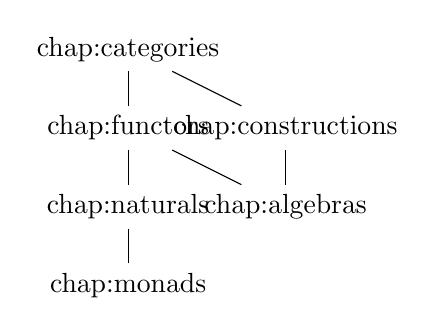
\begin{tikzpicture}
      \node (categories) {\nameref{chap:categories}};

      \node (functors) [below of=categories] {\nameref{chap:functors}};
      \node (naturals) [below of=functors]   {\nameref{chap:naturals}};
      \node (monads)   [below of=naturals]   {\nameref{chap:monads}};

      \node (constructions) [right of=functors,right of=functors] {\nameref{chap:constructions}};
      \node (algebras)      [below of=constructions]              {\nameref{chap:algebras}};

      \draw [-] (categories) to (functors);
      \draw [-] (functors)   to (naturals);
      \draw [-] (naturals)   to (monads);

      \draw [-] (categories)    to (constructions);
      \draw [-] (constructions) to (algebras);
      \draw [-] (functors)      to (algebras);
    \end{tikzpicture}
  \end{center}
  \caption{}
  \label{fig:overview}
\end{figure}

\todo{Each chapter has a similar structure. A motivation, theory, and
  Haskell. Some chapters include an analysis in Agda.}

\clearemptydoublepage
